\section{(0,2)序列采样器}\label{sec:(0,2)序列采样器}
\begin{remark}
    本节含有高级内容,第一次阅读时可以跳过。
\end{remark}

另一个生成高质量样本的方法是利用某些低偏差序列的显著性质
即允许我们满足两个想要的样本性质(其中仅一个用\refvar{StratifiedSampler}{}满足了):
它们为图像样本的一个像素值生成样本向量使得每个像素样本的样本值都彼此间分布良好,
同时该像素中所有像素样本的样本值集合也整体上分布良好。

该序列使用Sobol\footnote{\protect\refsec{Sobol采样器}的\refvar{SobolSampler}{}使用了
    Sobol序列的所有维度。}推导出的低偏差序列的前两维。
该序列是一种特殊类型的低偏差序列,称为$(0,2)$序列。
$(0,2)$序列以非常常规的方式分层。例如,$(0,2)$序列中的前16个样本
满足来自\refsec{分层采样}中分层采样的分层约束,
意味着每个范围为$\displaystyle\left(\frac{1}{4},\frac{1}{4}\right)$的矩形中只存在一个样本。
然而它们还满足拉丁超立方约束,即在每个范围为$\displaystyle\left(\frac{1}{16},1\right)$和
$\displaystyle\left(1,\frac{1}{16}\right)$的矩形中只有一个样本。
此外,在每个范围为$\displaystyle\left(\frac{1}{2},\frac{1}{8}\right)$和
$\displaystyle\left(\frac{1}{8},\frac{1}{2}\right)$的矩形中只有一个样本。

\reffig{7.28}展示了划分域的所有可能,其中$(0,2)$序列前16个样本都满足分层性质。
从该模式中获取的每组含16个样本的后续序列也都满足这些分布性质。
\begin{figure}[htbp]
    \centering
    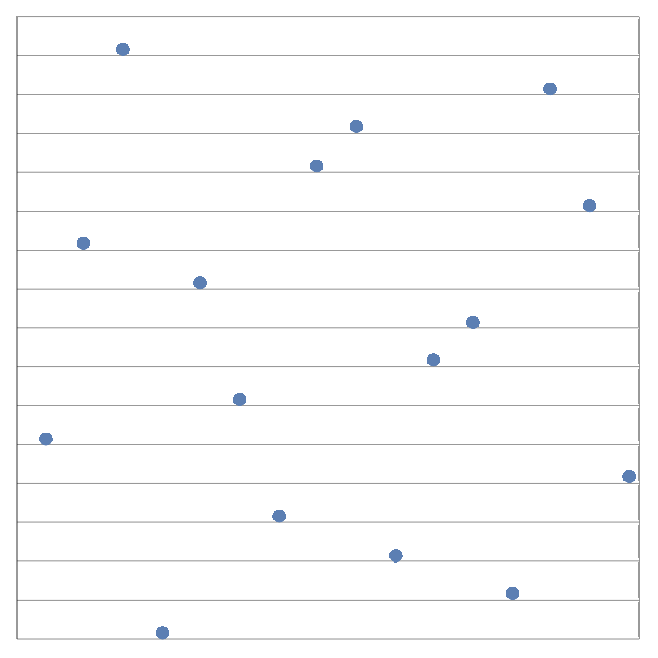
\includegraphics[width=0.49\linewidth]{chap07/elementary1x16.eps}\,
    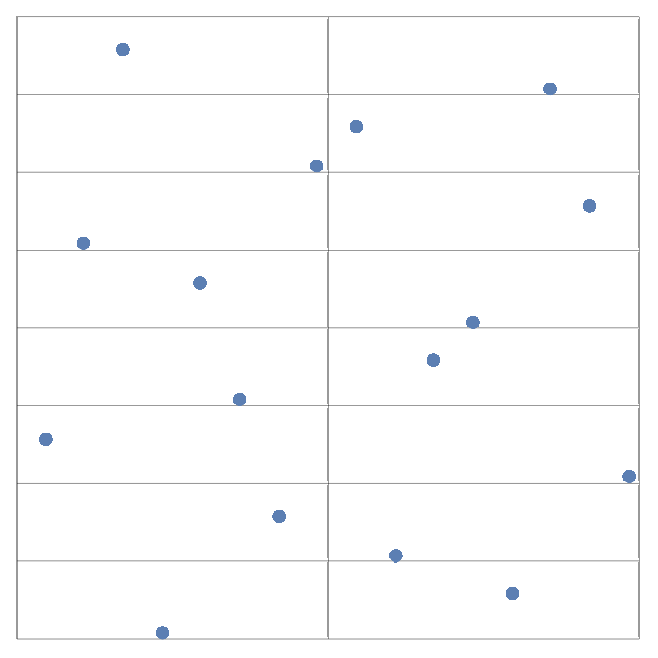
\includegraphics[width=0.49\linewidth]{chap07/elementary2x8.eps}\\
    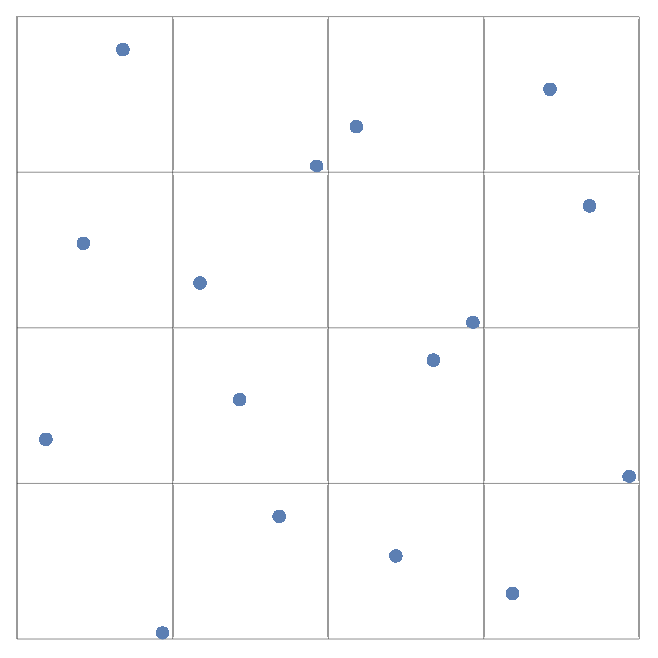
\includegraphics[width=0.49\linewidth]{chap07/elementary4x4.eps}\,
    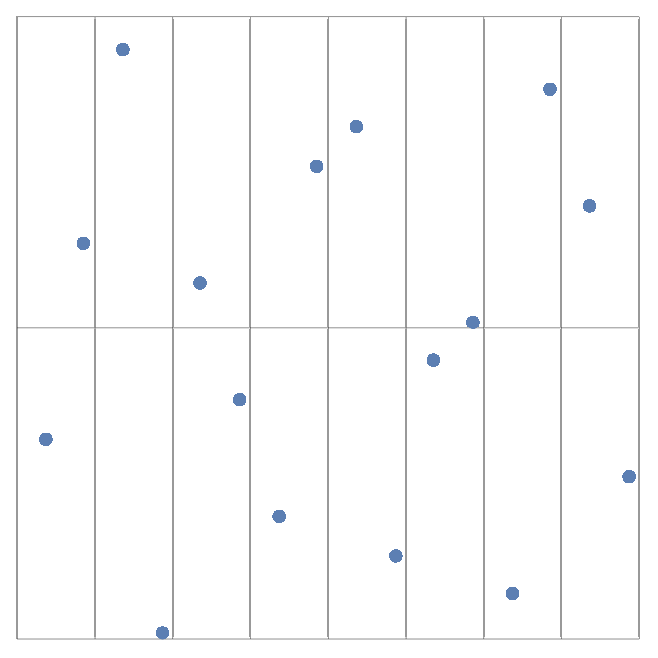
\includegraphics[width=0.49\linewidth]{chap07/elementary8x2.eps}\\
    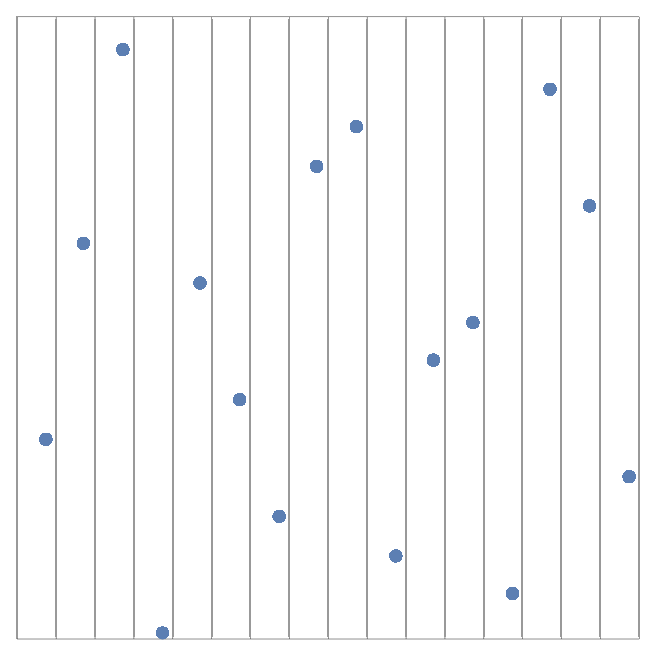
\includegraphics[width=0.49\linewidth]{chap07/elementary16x1.eps}
    \caption{在所有以2为底数的基本区间中都只有单个样本的采样模式。
        它同时满足$4\times4$分层和拉丁超立方约束以及所示的其他两个分层约束。}
    \label{fig:7.28}
\end{figure}

通常任何来自$(0,2)$序列的长为$2^{l_1+l_2}$的序列(其中$l_i$为非负整数)
都满足该一般分层约束。以2为底的两维的\keyindex{基本区间}{elementary interval}{}定义为
\begin{align*}
    E=\left\{\left[\frac{a_1}{2^{l_1}},\frac{a_1+1}{2^{l_1}}\right)\times\left[\frac{a_2}{2^{l_2}},\frac{a_2+1}{2^{l_2}}\right)\right\}\, ,
\end{align*}
其中整数$a_i=0,1,2\ldots,2^{l_i}-1$.
该序列中前$2^{l_1+l_2}$个值中的每一个样本都在相应基本区间中。
此外,后续每$2^{l_1+l_2}$个值构成的集合也满足同样的性质。

现在为了理解怎样把$(0,2)$序列应用于生成2D样本,
考虑有$2\times2$图像样本的像素,每个含$4\times4$个2D样本构成的数组。
依据相应的基本区间集,$(0,2)$序列前$(2\times2)\times(4\times4)=2^6$个值相互之间分布良好。
此外依据其相应的基本区间,前$4\times4=2^4$个样本自己也分布良好,
其后的$2^4$个也是这样,以此类推。因此,我们可以为一个像素的
首个图像样本的$4\times4$数组样本使用前16个$(0,2)$序列样本,
然后下一个图像样本用接下来的16个,以此类推。
结果是分布非常良好的样本点集。

\subsection{用生成器矩阵采样}\label{sub:用生成器矩阵采样}
比起\refvar{HaltonSampler}{},Sobol序列基于不同的样本点生成机制,
它在各维度上使用了倒根。即使将倒根函数中的整数除法转化为乘法和位移,
高质量高分辨率渲染所需的计算数十亿样本的计算量也会很大。
大部分计算开销来自于在天生是2进制的计算机上执行不以2为底的计算
(考虑代码片\refcode{Compute base-2 radical inverse}{}和模板函数\refvar{RadicalInverseSpecialized}{()}间的差别)。
